\section{Model Preparation}
\label{sec:assumptions}

\subsection{Assumptions}
\label{subsec:assumptions}

\hspace*{\parindent}To simplify the problem and make it convenient for us to simulate real-life conditions, we make the following basic assumptions, each of which is properly justified.

\begin{itemize}
    \item \textbf{Assumption 1:} The battery is treated as a single lumped thermal mass with uniform temperature distribution, ignoring internal temperature gradients.\\
    \textbf{Justification:} Modern smartphone batteries typically use thin, high-thermal-conductivity aluminum-plastic films or aluminum alloy casings with tightly packed internal cells. This structure results in extremely high heat conduction efficiency. Under conventional charging and discharging rates, the internal temperature difference is minimal, allowing the battery to be approximated as an isothermal system.

    \item \textbf{Assumption 2:} The model considers only the battery's normal operating state within a safe range and does not address abnormal failure modes such as overcharging, over-discharging, or short circuits.\\
    \textbf{Justification:} Modern smartphones are equipped with sophisticated Battery Management Systems (BMS) featuring strict protection mechanisms for voltage, current, and temperature. In normal usage scenarios, the BMS effectively prevents the device from exceeding safety boundaries. Therefore, this model focuses on normal battery depletion rather than sudden catastrophic failures.

    \item \textbf{Assumption 3:} The State of Health (SOH) of the battery is assumed to remain constant during short-term discharge simulations and prediction periods.\\
    \textbf{Justification:} Lithium-ion battery aging is a long-term electrochemical process typically measured in months or years. In a single discharge cycle or a short-period simulation (e.g., 24--48 hours), the daily variation in SOH is usually less than 0.01\%. Its impact on immediate Time-to-Empty predictions is negligible, justifying its treatment as a slowly varying parameter.

    \item \textbf{Assumption 4:} It is assumed that the amount of charge released during the discharge process is equal to the amount of charge input during the preceding charge process.\\
    \textbf{Justification:} Major energy losses in lithium-ion batteries typically occur during the charging phase (e.g., due to polarization internal resistance and heat generation from side reactions). For discharge modeling, particularly for State of Charge (SOC) estimation, ignoring minor losses from the charging phase regarding discharge capacity is acceptable within the range of engineering error.

    \item \textbf{Assumption 5:} The model for idle periods focuses solely on pure discharge behavior, temporarily excluding the interference of the charging process on the idle state.\\
    \textbf{Justification:} Accurately characterizing self-discharge and background power consumption in static scenarios while accounting for the complex dynamics of charge-discharge cycles is difficult. Since charging is not the primary factor in this context, the model focuses exclusively on the pure discharge process to highlight the key drivers of battery drain.

    \item \textbf{Assumption 6:} The power consumption of various smartphone hardware components (CPU, screen, RF, etc.) is modeled as a function of their Utilization Level.\\
    \textbf{Justification:} Extensive empirical research indicates a stable linear or non-linear relationship between the power consumption of smartphone components and their load rates. Therefore, modeling based on utilization functions is an effective method for characterizing power usage.

    \item \textbf{Assumption 7:} Ambient temperature, humidity, and air pressure are assumed to be known quantities or obtainable in real-time via sensors.\\
    \textbf{Justification:} Mainstream smartphones incorporate high-precision environmental sensor arrays. In extreme cases where sensors are absent, standard indoor environmental parameters (e.g., 25$^\circ$C, 1 atm) serve as reasonable default values for the model without affecting the overall prediction trends.
\end{itemize}

\subsection{Notations}
\label{subsec:notation}

\begin{table}[H]
    \centering
    \caption{Notations Table}
    \label{tab:notations}
    \begin{tabular}{@{}ll@{}}
        \toprule
        \textbf{Notations} & \textbf{Definition} \\
        \midrule
        $\SOC(t)$ & State of Charge at time $t$, representing battery level \\
        $\SOH(t)$ & State of Health, representing battery degradation level \\
        $V_{OC}$ & Open Circuit Voltage of the battery \\
        $V_{RC1}, V_{RC2}$ & Voltage across RC branches in the equivalent circuit \\
        $T(t)$ & Battery temperature at time $t$ \\
        $\Tamb$ & Ambient temperature \\
        $I(t)$ & Discharge current at time $t$ \\
        $\Qnom$ & Nominal battery capacity \\
        $R_0$ & Ohmic internal resistance \\
        $R_1, R_2$ & Polarization resistances in RC branches \\
        $C_1, C_2$ & Polarization capacitances in RC branches \\
        $\tau_1, \tau_2$ & Time constants of RC branches ($\tau_i = R_i C_i$) \\
        $K_0, K_1, K_2, K_3$ & Coefficients in the OCV-SOC Shepherd model \\
        $P(t)$ & Total power consumption at time $t$ \\
        $B$ & Screen brightness level (0--1) \\
        $U_{CPU}$ & CPU utilization level (0--1) \\
        $P_{net}$ & Network power consumption \\
        $t_{empty}$ & Time-to-empty, battery discharge duration \\
        $S_1, S_T$ & First-order and total-order Sobol sensitivity indices \\
        \bottomrule
    \end{tabular}
\end{table}

\begin{figure}[H]
    \centering
    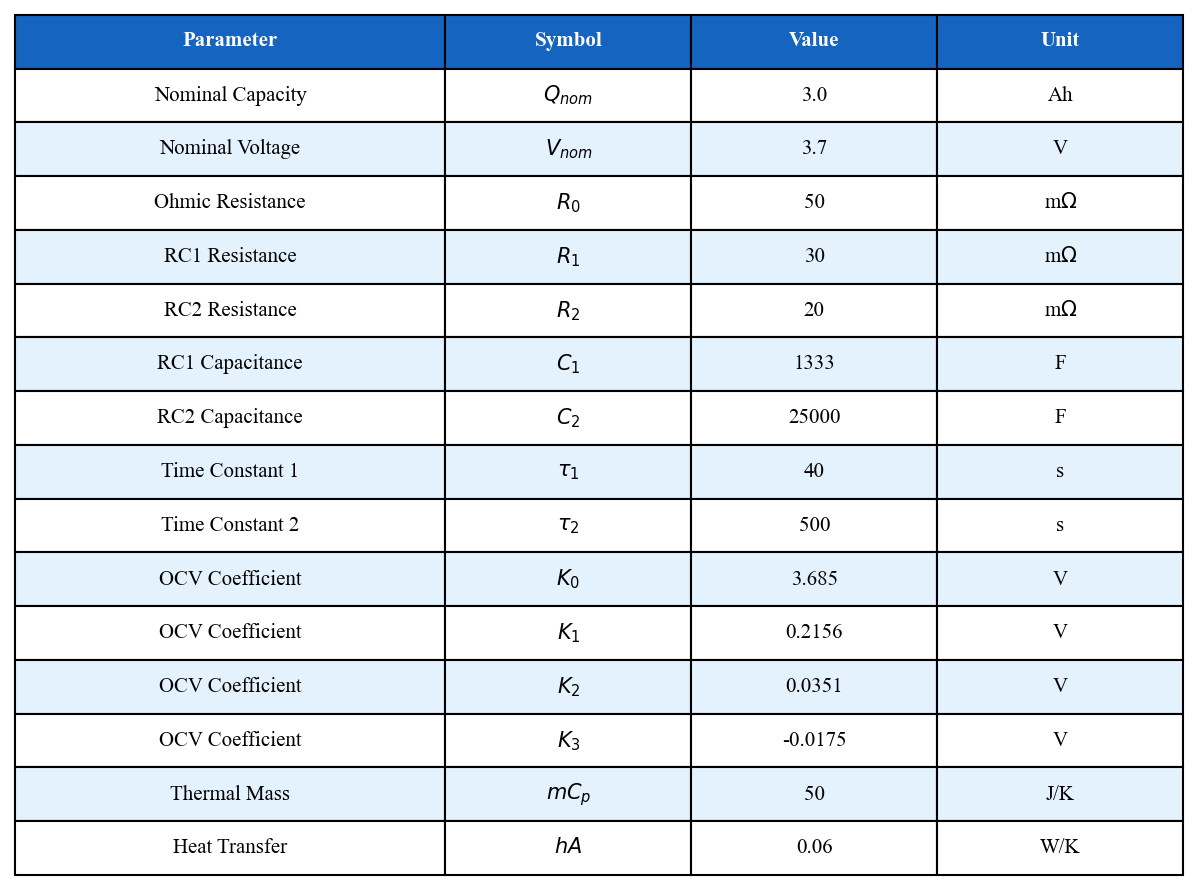
\includegraphics[width=0.85\textwidth]{figures/figure/8BA9C2DF287E6F1A95182819D12CDD73.png}
    \caption{Battery model parameters summary. This table presents the key electrical and thermal parameters used in the 2-RC equivalent circuit model, including nominal capacity, voltage, ohmic and polarization resistances, RC time constants, OCV coefficients, and thermal properties.}
    \label{fig:battery_parameters}
\end{figure}

\subsection{Data Sources}
\label{subsec:data}

\begin{itemize}
    \item \textbf{Battery Specifications:} Manufacturer datasheets for standard smartphone Li-ion cells, specifically the LG 18650HG2 (3.0 Ah, 3.6V nominal) \cite{LG18650HG2} and Panasonic 18650PF \cite{Panasonic18650PF}.
    \item \textbf{ECM Parameters:} Electrochemical Impedance Spectroscopy (EIS) and Hybrid Pulse Power Characterization (HPPC) data acquired from Mendeley Data repositories \cite{MendeleyEIS}.
    \item \textbf{OCV--SOC Characterization:} Low-current (C/20) discharge tests and incremental current OCV data used to parameterize the nonlinear Shepherd model \cite{Plett2004OCV}.
    \item \textbf{Power Consumption:} Validated component-level power models (CPU, Display, Network) derived from power measurement studies \cite{UCSD3W, Carroll2010, Pathak2012}.
    \item \textbf{Aging Data:} Long-term cycling capacity fade and impedance growth measurements from the NASA PCoE Prognostics Data Repository \cite{NASAPCoE} and Oxford Battery Degradation Dataset \cite{OxfordBattery}.
    \item \textbf{Validation Data:} Dynamic drive cycle profiles (UDDS, HWFET, LA92, US06) \cite{UDDS, HWFET} and mixed usage scenarios used for model verification and error analysis.
\end{itemize}

To ensure data quality and model robustness, we performed rigorous preprocessing on the raw datasets. First, variable-rate time-series data from HPPC and drive cycle tests were resampled to a uniform 0.1s interval to align timestamps. For OCV characterization, we calculated the State of Charge (SOC) via Ampere-hour integration and clamped values to the interval [0.001,0.999] to prevent logarithmic singularities during Shepherd model fitting. We applied a moving average filter to raw voltage measurements to mitigate sensor noise and utilized derivative thresholding to precisely identify current pulse boundaries for resistance extraction. Additionally, empirical power curves extracted from literature were digitized, fitted to nonlinear functions, and normalized to a standard 3.0 Ah capacity to ensure consistency across different simulation scenarios.